\documentclass[a4paper,10pt] {article}
\usepackage[top=3cm,left=3cm,right=2cm,bottom=2cm]{geometry} % definir margens da página %
\usepackage[utf8]{inputenc} % suporte a acentos %
\usepackage{graphicx} % incluir figuras %
\usepackage[portuguese]{babel}

\begin{document}

\begin {center}
UNIVERSIDADE FEDERAL DO RIO GRANDE DO SUL

Programa de Pós-Graduação em Computação - PPGC

Concepção de Circuitos VLSI - CMP115

Professor Sergio Bampi

Aluno: Daniel Munari Palomino 

\vspace{7mm}
\textbf{ TRABALHO PRÁTICO 3 - \textit{XOR} }
\vspace{7mm}

\end{center}

\section{Objetivo}
Projetar o \textit{layout} de uma porta lógica XOR de duas entradas considerando duas implementações diferentes: (1) CMOS estática com 12 transistores e (2) Transistor de Passagem com 6 transistores. Além disso, realizar a caracterização elétrica dos \textit{layouts} e gerar os seguintes resultados:

\begin{itemize}
\item Valores dos tempos de resposta para as duas xor projetadas ($Tp_{hl}$, $Tp_{lh}$, $T_{rise}$ e $T_{fall}$).
\item Medir a potência média consumida.
\item Calcular a energia média consumida.

\end{itemize}

\section{Desenvolvimento}

Primeiramente foram desenvolvidos os \textit{layouts} referentas as duas versões da porta XOR de duas entradas especificadas pelo trabalho.
As figuras \ref{fig:xorStaticLayout} e \ref{fig:xorTransLayout} apresentam o layout da porta XOR estática CMOS e da porta XOR com transistor de passagem,
respectivamente. O desenvolvimento destes leyouts foi realizado utilizando a ferramenta Virtuoso da Cadence.

\begin{figure}[h]
  \begin{minipage} [b] {0.48 \linewidth}
	\centering
	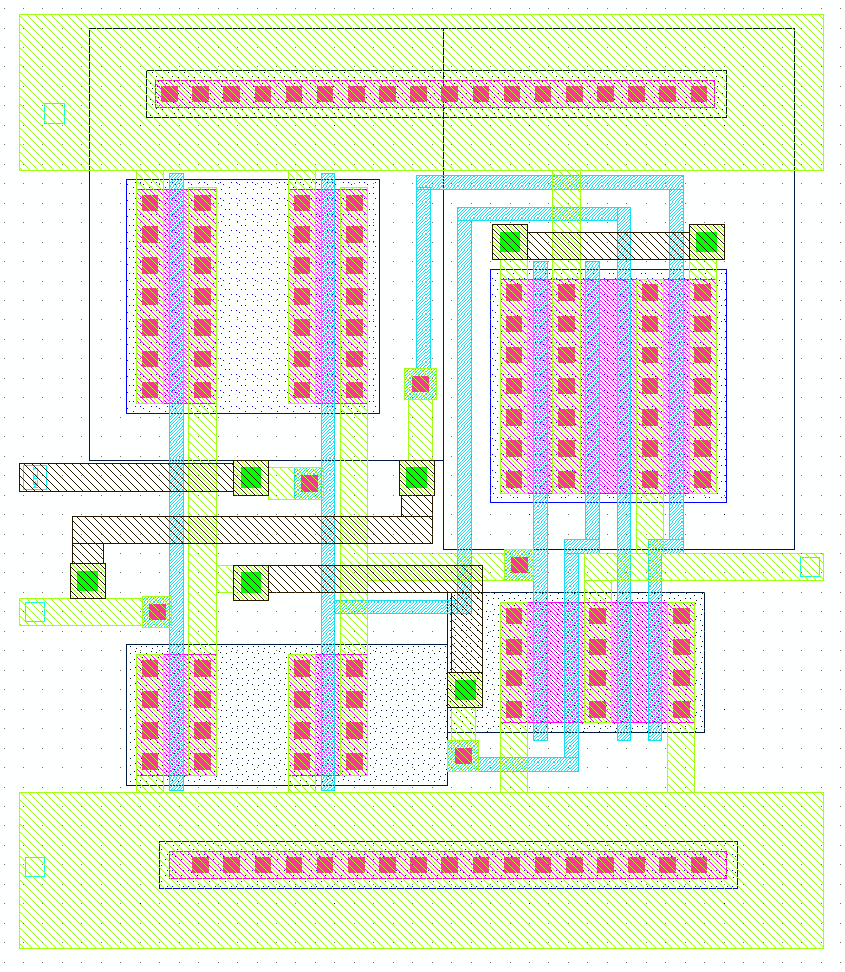
\includegraphics[scale=0.25]{xorStaticCMOSlayout.png}
	\caption{Layout da porta XOR estática CMOS.}
	\label{fig:xorStaticLayout}
  \end{minipage}
  \begin{minipage} [b] {0.48 \linewidth}
	\centering
	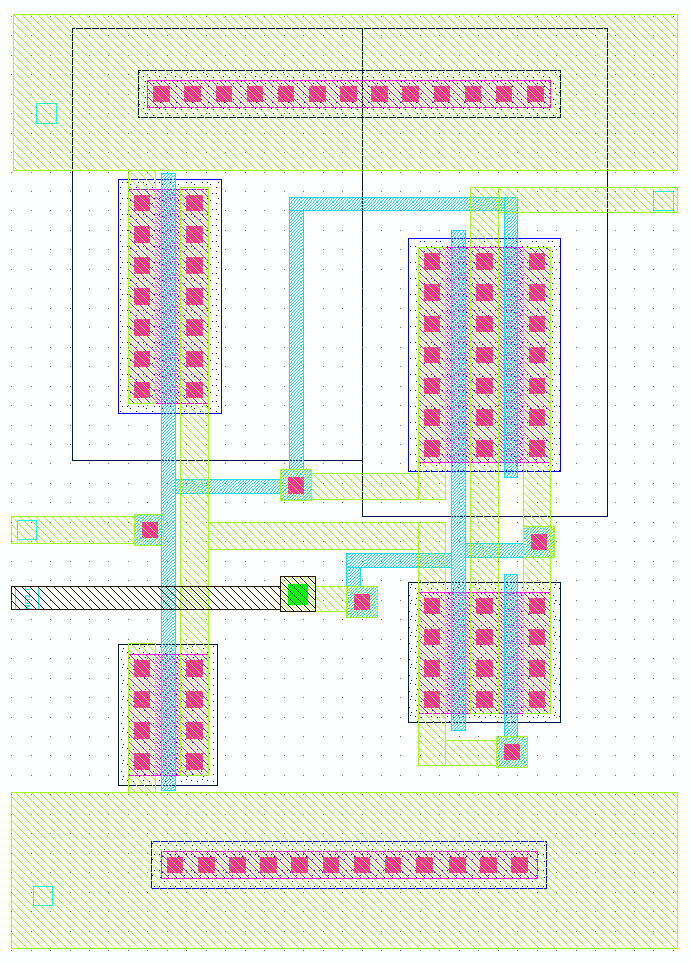
\includegraphics[scale=0.25]{xorTransGatelayout.png}
	\caption{Layout da porta XOR com Transistor de Passagem.}
	\label{fig:xorTransLayout}
  \end{minipage}
\end{figure}

A largura dos transistores utilizada foi de 5.5$\mu$ para os transitores PMOS e 3.1$\mu$ para os transistores NMOS.
As figuras \ref{fig:xorStaticSchematic} e \ref{fig:xorTransSchematic} mostram os diagramas esquemáticos projetados de acordo com as duas implementações de XOR propostas.

\begin{figure}[h]
  \begin{minipage} [b] {0.48 \linewidth}
	\centering
	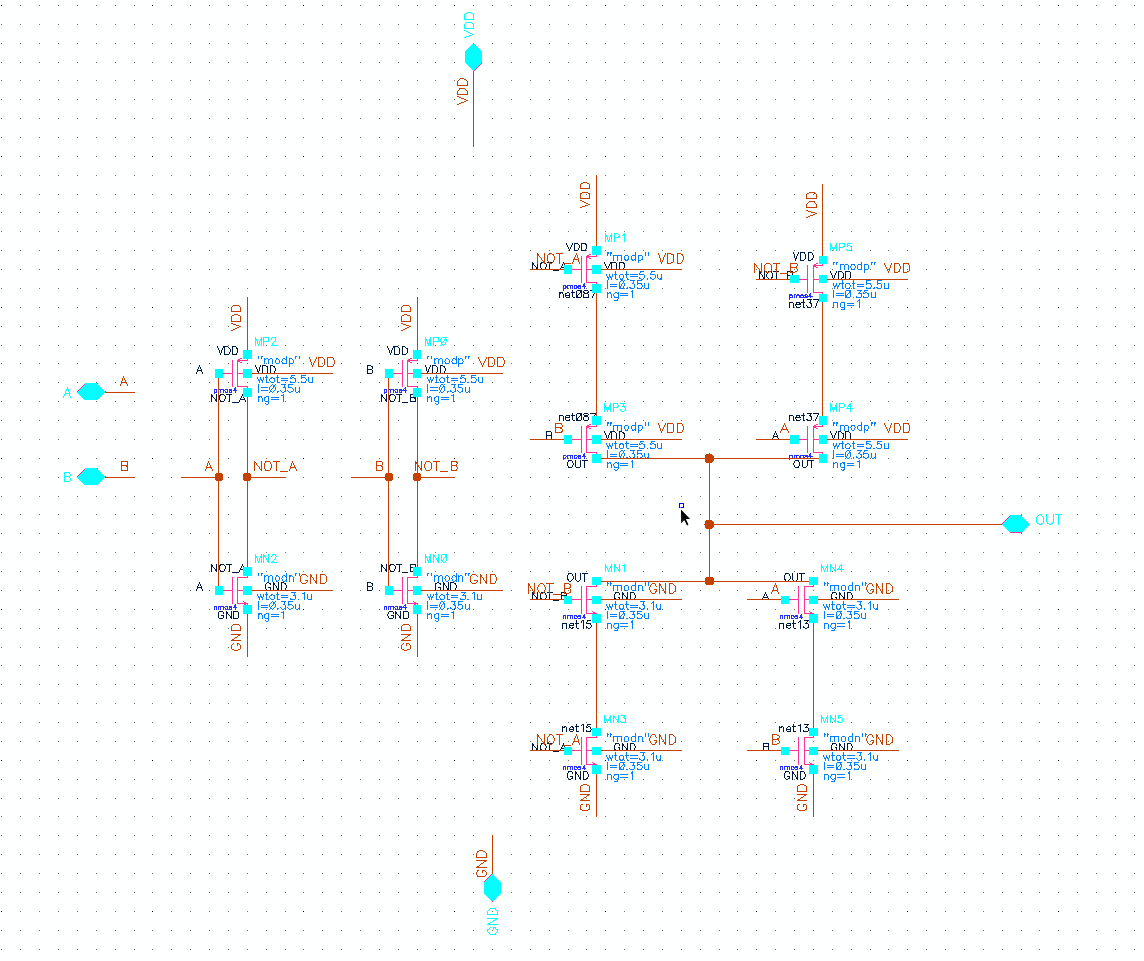
\includegraphics[scale=0.2]{xorStaticCMOSSchematic.png}
	\caption{Diagrama esquemático da porta XOR estática CMOS.}
	\label{fig:xorStaticSchematic}
  \end{minipage}
  \begin{minipage} [b] {0.48 \linewidth}
	\centering
	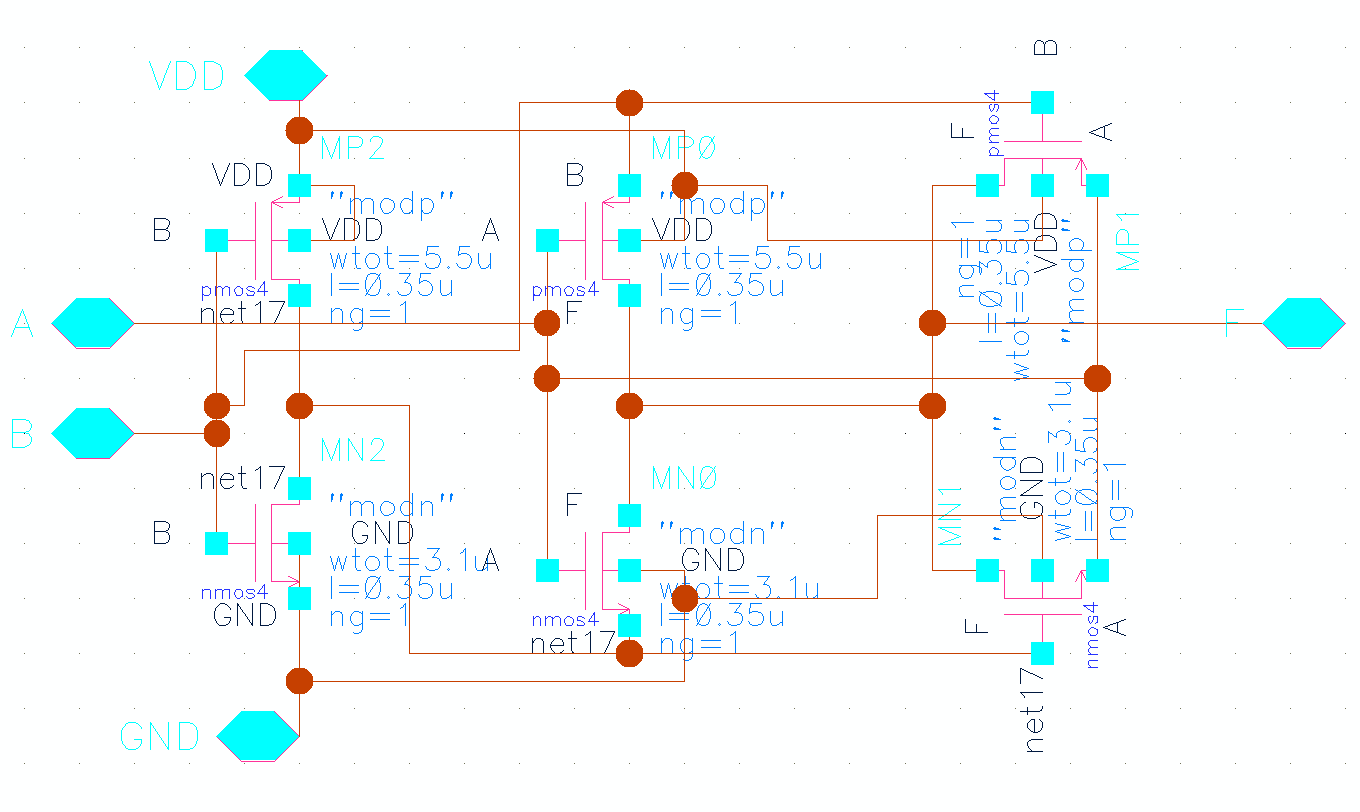
\includegraphics[scale=0.2]{xorTransGateSchematic.png}
	\caption{Diagrama esquemático da porta XOR com Transistor de Passagem.}
	\label{fig:xorTransSchematic}
  \end{minipage}
\end{figure}

\section{Verificações}
\label{sec:veri}

A verificação DRC e LVS (\textit{Layout versus Schematic} sobre os layouts projetados foram realizadas de acordo com as regras de layout da tecnologia AMS 0.35$\mu$.

As figuras \ref{fig:xorStaticDRC}, \ref{fig:xorTransDRC}, \ref{fig:xorStaticLVS} e \ref{fig:xorTransLVS} mostram, respectivamente, a saída do software virtuoso para
a verificação DRC e LVS de cada uma das versões da XOR de duas entradas desenvolvidas.

\begin{figure}[h]
  \begin{minipage} [b] {0.48 \linewidth}
	\centering
	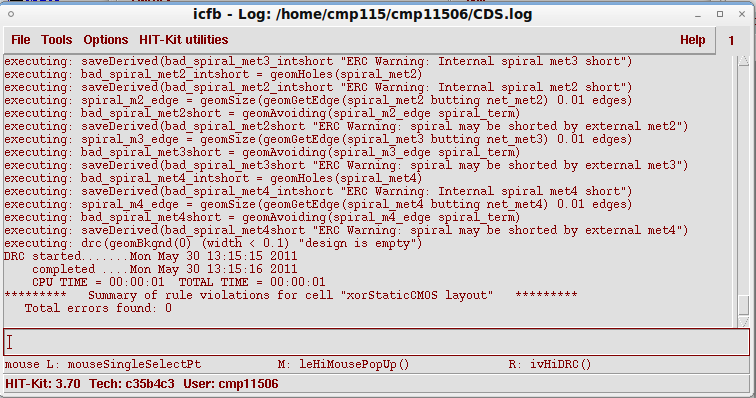
\includegraphics[scale=0.25]{xorStaticCMOSdrc.png}
	\caption{Verificação DRC para a porta XOR estática CMOS.}
	\label{fig:xorStaticDRC}
  \end{minipage}
  \begin{minipage} [b] {0.48 \linewidth}
	\centering
	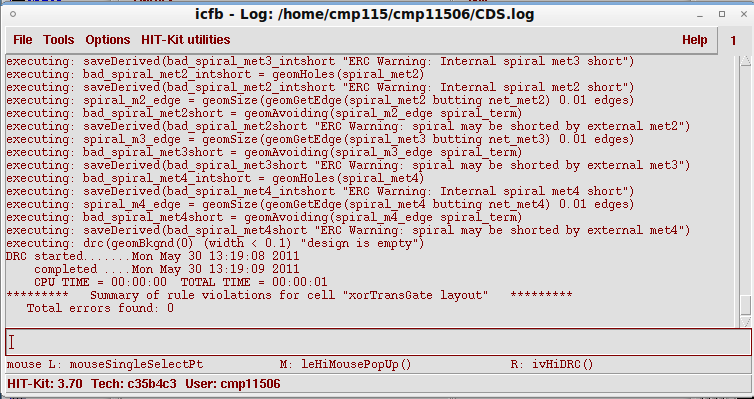
\includegraphics[scale=0.25]{xorTransGatedrc.png}
	\caption{Verificação DRC para a porta XOR com Transistor de Passagem.}
	\label{fig:xorTransDRC}
  \end{minipage}
\end{figure}

\begin{figure}[h]
  \begin{minipage} [b] {0.48 \linewidth}
	\centering
	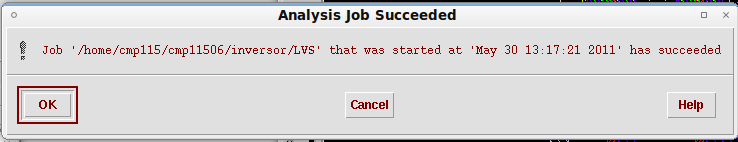
\includegraphics[scale=0.27]{xorStaticCMOSlvs.png}
	\caption{Verificação LVS para a porta XOR estática CMOS.}
	\label{fig:xorStaticLVS}
  \end{minipage}
  \begin{minipage} [b] {0.48 \linewidth}
	\centering
	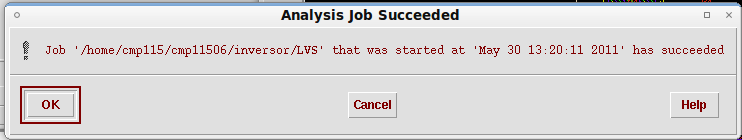
\includegraphics[scale=0.27]{xorTransGateLvs.png}
	\caption{Verificação LVS para a porta XOR com Transistor de Passagem.}
	\label{fig:xorTransLVS}
  \end{minipage}
\end{figure}

A extração das capacitâncias parasitas também foi realizada afim de poder realizar a verificação LVS. Além disso,
os \textit{layouts} com as capacitâncias parasitas extraídas foram utilizados para realizar a caracterização elétrica de cada uma das duas versões de porta XOR de duas entradas implementadas.
Essa caracterizacao elétrica será apresentada na próxima seção.

As figuras \ref{fig:xorStaticExtracted} e \ref{fig:xorTransExtracted} apresentam os \textit{layouts} com as capacitâncias parasitas extraídas para a versão de porta XOR de duas entradas
estática CMOS e para a versão com transistor de passagem, respectivamente.

\begin{figure}[h]
  \begin{minipage} [b] {0.48 \linewidth}
	\centering
	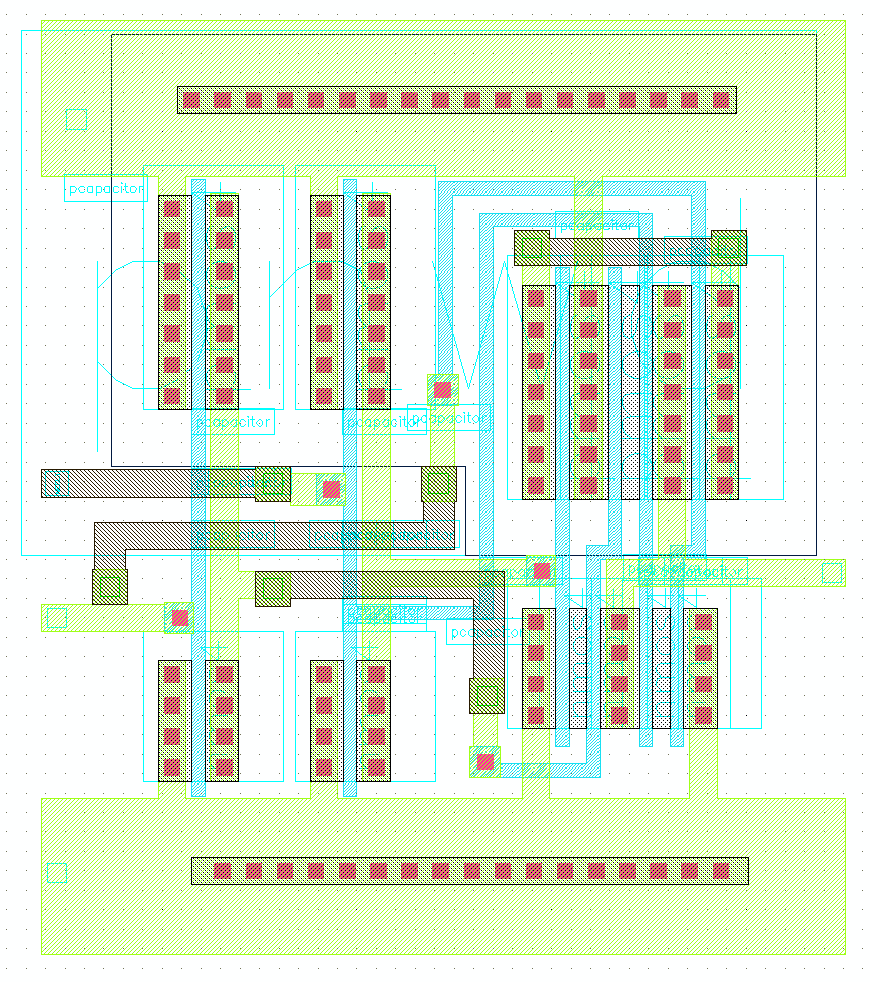
\includegraphics[scale=0.2]{xorStaticCMOSextracted.png}
	\caption{Layout com as capacitâncias parasitas extraídas da porta XOR estática CMOS.}
	\label{fig:xorStaticExtracted}
  \end{minipage}
  \begin{minipage} [b] {0.48 \linewidth}
	\centering
	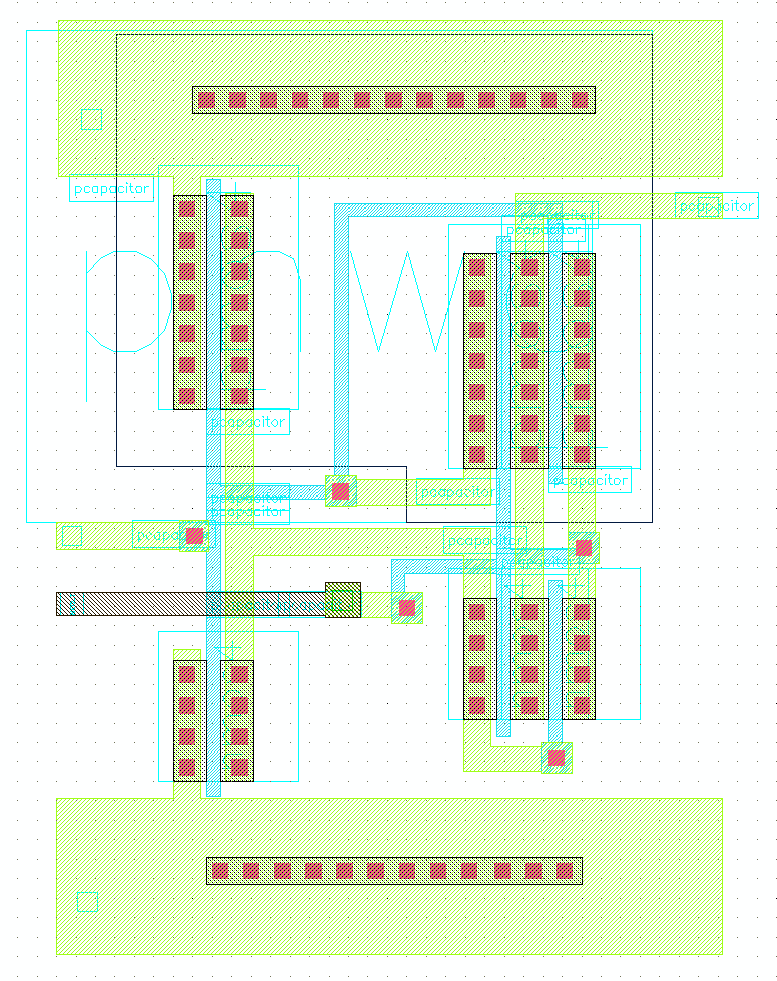
\includegraphics[scale=0.2]{xorTransGateExtracted.png}
	\caption{Layout com as capacitâncias parasitas extraídas da porta XOR com Transistor de Passagem.}
	\label{fig:xorTransExtracted}
  \end{minipage}
\end{figure}



\section{Caracterização Elétrica}
\label{sec:caracterizacao}
O modelo de simulação utilizado para as duas implementações da porta XOR de duas entradas está representado na figura \ref{fig:xorTest}. A carga utilizada na saída foi de $0,1pF$.

\begin{figure}[h]
	\centering
	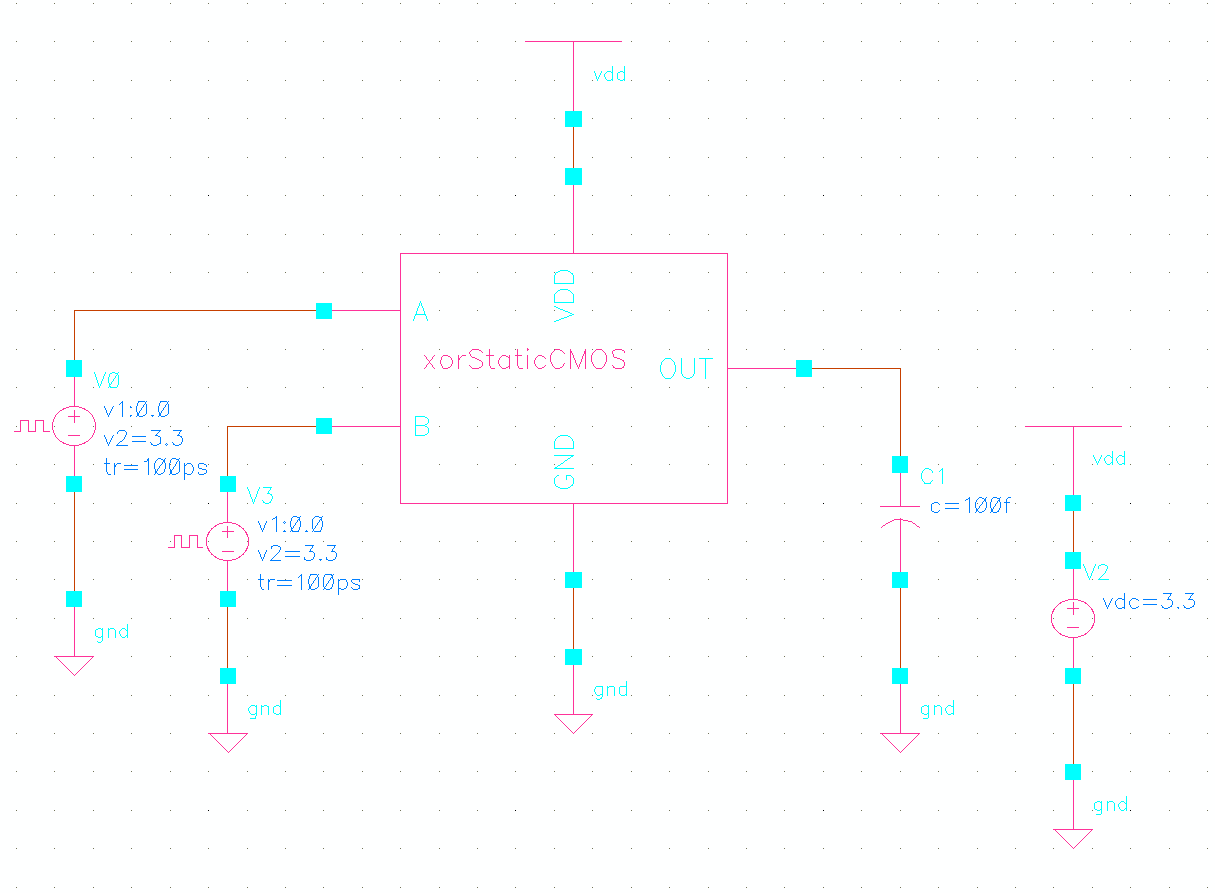
\includegraphics[scale=0.25]{xorStaticCMOStest.png}
	\caption{Modelo de simulação utilizado para realizar a caracterizacao elétrica das portas XOR projetadas.}
	\label{fig:xorTest}
\end{figure}

Considerando a ánalise transiente realizada, quatro tempos de resposta foram obtidos: (1)$Tp_{hl}$ (tempo de high low),
(2$)Tp_{lh}$ (tempo de low high), (3)$T_{rise}$ (tempo de subida) e (4)$T_{fall}$ (tempo de descida).
Para medir corretamente esses tempos de resposta, foi necessário considerar todas as transições possíveis na entrada.
As tabelas \ref{tab:table1} e \ref{tab:table2} mostram os tempos medidos para a XOR estática CMOS e com transistor de passagem respectivamente.
Em destaque os tempos de resposta considerando o pior caso.3

\begin{table} [h]
  \centering
  \caption{Transições e tempos de resposta para a XOR estática CMOS.}
  \begin{tabular}{c|c|c|c|c|c|c|c}
    \hline
    A & B & A' & B' & Trise (ns) & Tfall (ns) & TPlh (ns) & TPhl(ns) \\ \hline
    1 & 1 & 0 &  1  & 0,777 & - & 0,361 & - \\ \hline
    1 & 1 & 1 &  0  & 0,832 & - & 0,36 & - \\ \hline
    0 & 0 & 1 &  0  & \bf{0,847} & - & \bf{0,46} & - \\ \hline
    0 & 0 & 0 &  1  & 0,776 & - & 0,428 & - \\ \hline
    0 & 1 & 1 &  1  & - & 0,407 & - & 0,222 \\ \hline
    0 & 1 & 0 &  0  & - & 0,496 & - & \bf{0,342} \\ \hline
    1 & 0 & 0 &  0  & - & \bf{0,497} & - & 0,329 \\ \hline
    1 & 0 & 1 &  1  & - & 0,406 & - & 0,219 \\ \hline
  \end{tabular}
  \label{tab:table1}
\end{table}

\begin{table} [h]
  \centering
  \caption{Transições e tempos de resposta para a XOR com transistor de passagem.}
  \begin{tabular}{c|c|c|c|c|c|c|c}
    \hline
    A & B & A' & B' & Trise (ns) & Tfall (ns) & TPlh (ns) & TPhl(ns) \\ \hline
    1 & 1 & 0 &  1  & 0,4 & - & 0,361 & - \\ \hline
    1 & 1 & 1 &  0  & 0,353 & - & 0,36 & - \\ \hline
    0 & 0 & 1 &  0  & 0,35 & - & \bf{0,46} & - \\ \hline
    0 & 0 & 0 &  1  & \bf{0,401} & - & 0,428 & - \\ \hline
    0 & 1 & 1 &  1  & - & 0,419 & - & 0,221 \\ \hline
    0 & 1 & 0 &  0  & - & 0,26 & - & 0,116 \\ \hline
    1 & 0 & 0 &  0  & - & 0,227 & - & 0,085 \\ \hline
    1 & 0 & 1 &  1  & - & \bf{0,419} & - & \bf{0,261} \\ \hline
  \end{tabular}
  \label{tab:table2}
\end{table}

O passo seguinte foi realizar a medição da potência consumida pelas duas versões da porta XOR projetada.
O modelo de simulação mostrado na figura  também foi utilizado nesta etapa. A frequência de chaveamento utilizada foi de 200MHz.

A potência consumida foi de 0,355mW para a versão estática CMOS e 0,045mW para a versão com transistor de passagem. Sendo assim, a energia média consumida foi de 3,55pJ para a XOR estática
CMOS e 0.45pj para a XOR com transistor de passagem. A tabela \ref{tab:table3} apresenta uma comparação considerando todos os resultados obtidos para as duas versões.

\begin{table} [h]
  \centering
  \caption{Comparação entre as duas implementações de XOR de duas entradas.}
  \begin{tabular}{c|c|c|c|c|c|c|c}
    \hline
		& Trise (ns)	& Tfall (ns)	& TPlh (ns)	& TPhl(ns)	& Tp(ns)	& Potência(mW)	& Energia \\ \hline
    CMOS	& 0,847 	& 0,497		& 0.46		& 0,342		& 0,401		& 0,355		& 3.55pJ  \\ \hline
    Passagem	& 0,401		& 0,419		& 0,46		& 0,261		& 0,365		& 0,045		& 0,45pJ  \\ \hline
  \end{tabular}
  \label{tab:table3}
\end{table}

\section{Referências}
\begin{enumerate}
\item Rabaey, J., Chandrakasan, \textordfeminine,Nikolic, B. - "Digital Integrated Circuits - A Design Perspective". Prentice Hall, 2\textordfeminine Edição. ISBN 0-13178609-1.
\item AMS 0.35$\mu$m CMOS C35 Design Rules revisão 2.0, 2003.
\end{enumerate}

\end{document}
